

%%%%%%%%%%%%%%%%%%%%%%%%%%%%%%%%%%%%%%%%%%%%%%%%%%%%%%%%%%%%%%%%%%%%%%%%%%%%
%%%%%%%%%%%%%%%%%%%%%%%%%%%%%%%%%%%%%%%%%%%%%%%%%%%%%%%%%%%%%%%%%%%%%%%%%%%%
%%%%%%%%%%%%%%%%%%%%%%%%%%%%%%%%%%%%%%%%%%%%%%%%%%%%%%%%%%%%%%%%%%%%%%%%%%%%

\begin{frame}[t]{Which estimators do we study?}

\textbf{Z-estimators.  }
Suppose we have $N$ data points $\dvec = \d_{1}, \ldots, \d_{N}$.  Then:
%
\begin{align*}
%
\thetahat :=
\thetavec \,\, \textrm{ such that } \,\,
\sumn
G(\thetavec, \d_{n}) =  \zP .
%
\end{align*}
%
% These are ``Z-estimators,'' i.e., roots of estimating equations.
%
\textbf{Examples:} MLE, OLS, VB, \&c (all minimizers of smooth empirical loss).

\hrulefill

% \vspace{1em}
\textbf{Function of interest.  }Qualitative decision
based on $\thetafun(\thetahat) \in \mathbb{R}$.  E.g.:
%\textbf{Examples:}
\begin{itemize}
\item A particular component: $\thetafun(\theta) = \theta_d$
\item The end of a confidence interval:
    $\thetafun(\theta) = \theta_d + \frac{1.96}{\sqrt{N}} \hat\sigma(\thetahat)$
\end{itemize}

\hrulefill

Fix a proportion $0 < \alpha \ll 1$ of points to drop and
%
find a set $\nset \subset \left\{1, \ldots N\right\}$ with $|\nset| \le
\alphan$ that extremizes $\thetafun(\thetahat)$ when dropped.
%
%
\begin{itemize}
    \item \textbf{Problem: }  There are many sets with $|\nset| \le \alphan$.
        \begin{itemize}
        \item E.g., in \citet{angelucci2015microcredit},
            ${16,560 \choose 15} \approx 1.5 \cdot 10^{51}$
        \end{itemize}
    \item \textbf{Problem: } Evaluating $\thetafun(\thetahat(\dvec_{-\nset}))$
        requires an estimation problem.
        \begin{itemize}
        \item E.g., in \citet{angelucci2015microcredit} computing the OLS
            estimator.
        \item Other examples are even harder (VB, machine learning)
        \end{itemize}
\end{itemize}
%
\textbf{An approximation is needed!}
\end{frame}



%%%%%%%%%%%%%%%%%%%%%%%%%%%%%%%%%%%%%%%%%%%%%%%%%%%%%%%%%%%%%%%%%%%%%%%%%%%%
%%%%%%%%%%%%%%%%%%%%%%%%%%%%%%%%%%%%%%%%%%%%%%%%%%%%%%%%%%%%%%%%%%%%%%%%%%%%
%%%%%%%%%%%%%%%%%%%%%%%%%%%%%%%%%%%%%%%%%%%%%%%%%%%%%%%%%%%%%%%%%%%%%%%%%%%%

\begin{frame}[t]{Which estimators do we study?}
% Suppose we have $N$ data points $\d_{1}, \ldots, \d_{N}$.  Then:
%
\begin{align*}
%
\thetahat \only<2->{\color{red} (\w) \color{black}} :=
\vec\theta \,\, \textrm{ such that } \,\,
\sumn
\only<2->{ \color{red} \w_{n} \color{black}}
G(\vec\theta, \d_{n}) =  \zP .
%
\end{align*}
%
\begin{minipage}{0.45\textwidth}
\begin{center}
Original weights: $\onevec = (1,\ldots,1)$
    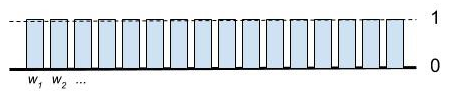
\includegraphics[width=1.0\textwidth]{static_figures/orig_weights}
Leave points out by setting their elements of $\w$ to zero.
    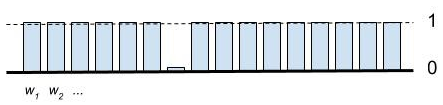
\includegraphics[width=1.0\textwidth]{static_figures/weights_loo}
\end{center}
\end{minipage}
\begin{minipage}{0.45\textwidth}
\begin{center}
    \begin{tikzpicture}
        \node[anchor=south west,inner sep=0] (image) at (0,0) {
            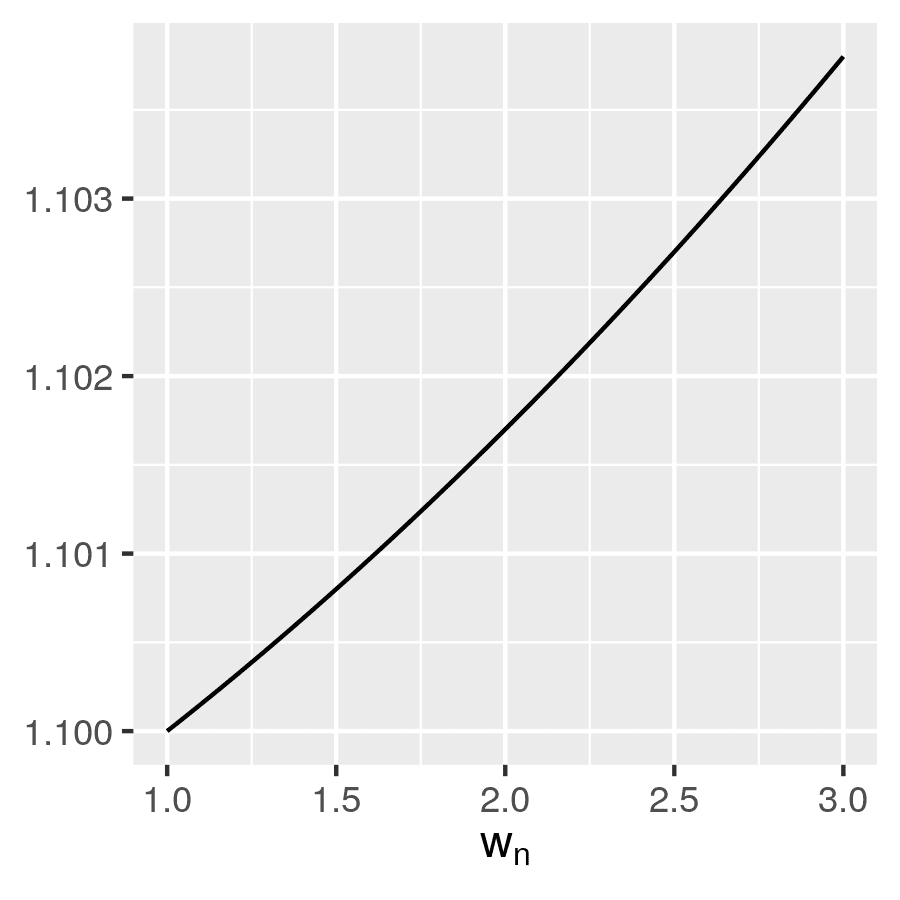
\includegraphics[width=0.88\textwidth]{static_figures/e_beta_w}
        };
        \begin{scope}[x={(image.south east)},y={(image.north west)}]
            \draw[blue, thick, <-] (0.2,0.23) -- ++(0.1,0.25)
                    node[above,black,fill=white]
                    {\small $\thetafun(\thetahat(\onevec))$};
            \draw[blue, thick, <-] (0.8,0.8) -- ++(-0.1,0.1)
                    node[left,black,fill=white]
                    {\small $\thetafun(\thetahat(\w))$};
            \draw[red, thick, -] (0.18,0.18) -- ++(1.2 * 0.6, 1.2 * 0.48);
            \draw[blue, thick, <-] (0.75,0.55) -- ++(0.02,-0.1)
                    node[below,black,fill=white]
                    {\small Slope $ = \infl_n$};
        \end{scope}
    \end{tikzpicture}
\end{center}
\end{minipage}

The slopes $\infl_n := \fracat{\partial \thetafun(\thetahat(\w))}{\partial \w_n}{\onevec}$ are values of the \textbf{empirical influence function}
\citep{hampel1986robustbook}.  We call them ``influence scores.''

% \vspace{1em}
% $\thetahat(\w)$ well-defined even for continuous values of the weights!

\vspace{1em}
Second-order derivatives control the error of
the linear approximation.

\end{frame}




%%%%%%%%%%%%%%%%%%%%%%%%%%%%%%%%%%%%%%%%%%%%%%%%%%%%%%%%%%%%%%%%%%%%%%%%%%%%
%%%%%%%%%%%%%%%%%%%%%%%%%%%%%%%%%%%%%%%%%%%%%%%%%%%%%%%%%%%%%%%%%%%%%%%%%%%%
%%%%%%%%%%%%%%%%%%%%%%%%%%%%%%%%%%%%%%%%%%%%%%%%%%%%%%%%%%%%%%%%%%%%%%%%%%%%


\begin{frame}{Taylor series approximation.}
%
\textbf{Problem: } How large can you make $\thetafun(\thetahat(\w))$
leaving out no more than $\alphan$ points?  \textbf{Combinatorially hard!}

\hrulefill

\vspace{1em}
To simplify the search over $\w$, we form the Taylor series approximation:
%
\begin{align*}
	\thetafun(\thetahat(\w))
		&\approx
        \color{red}
        \thetafunlin(\w)
        \color{black}
		:=  \thetafun(\thetahat(\onevec)) +
        \sumn \infl_n (\w_n -1)
        \color{black}
\end{align*}
%
\textbf{Approximate solution: } How large can you make $\thetafunlin(\w)$
leaving out no more than $\alphan$ points?  \textbf{Easy! }

\vspace{1em}
The most influential points for $\thetafunlin(\w)$ have the
most negative $\infl_n$.

\hrulefill

The $\infl_n$ are automatically computable using the
\textbf{implicit function theorem} and \textbf{automatic differentiation}.

\hrulefill

We provide \textbf{finite-sample theory} showing that
$\abs{\thetafun(\thetahat(\w)) - \thetafunlin(\w)} =
O\left(\vnorm{\frac{1}{N}(\w - \onevec)}^2_2\right) =
O\left(\alpha\right)$ as $\alpha \rightarrow 0$.

\end{frame}


%
% %%%%%%%%%%%%%%%%%%%%%%%%%%%%%%%%%%%%%%%%%%%%%%%%%%%%%%%%%%%%%%%%%%%%%%%
% %%%%%%%%%%%%%%%%%%%%%%%%%%%%%%%%%%%%%%%%%%%%%%%%%%%%%%%%%%%%%%%%%%%%%%%
% %%%%%%%%%%%%%%%%%%%%%%%%%%%%%%%%%%%%%%%%%%%%%%%%%%%%%%%%%%%%%%%%%%%%%%%
%
% \begin{frame}{Taylor series approximation.}
%
% \vspace{1em}
% \textbf{How to compute the influence scores $\infl_n$? }
%
%
% By the chain rule,
% $\infl_n = \fracat{\partial \thetafun(\thetahat(\w))}{\partial \w_n}{\onevec}
% = \fracat{\dee \thetafun(\theta)}
%     {\dee \theta^T}{\thetahat}
%   \fracat{\partial \thetahat(\w)}{\partial \w_n}{\onevec}$.
%
% Recall that
% %\begin{align*}
% %
% $\thetahat(\w) :=
% \vec\theta \,\, \textrm{ such that } \,\,
% \sumn \w_{n}  G(\vec\theta, \d_{n}) =  \zP$.
% %
% %\end{align*}
% %
%
% The \textbf{implicit function theorem} expresses $\fracat{\partial
% \thetahat(\w)}{\partial \w_n}{\onevec}$ as a linear system.
%
% \vspace{1em}
% Computation of $\infl_n$ is fully automatible from a
% software implemenation of $G(\cdot, \cdot)$ and $\thetafun(\cdot)$ with
% \textbf{automatic differentiation}
% \citep{baydin2017automatic}.
%
% \vspace{1em}
% We have an \texttt{R} package, \texttt{rgiordan/zaminfluence},
% for OLS and IV.
%
% \end{frame}



%%%%%%%%%%%%%%%%%%%%%%%%%%%%%%%%%%%%%%%%%%%%%%%%%%%%%%%%%%%%%%%%%%%%%%%%%%%%
%%%%%%%%%%%%%%%%%%%%%%%%%%%%%%%%%%%%%%%%%%%%%%%%%%%%%%%%%%%%%%%%%%%%%%%%%%%%
%%%%%%%%%%%%%%%%%%%%%%%%%%%%%%%%%%%%%%%%%%%%%%%%%%%%%%%%%%%%%%%%%%%%%%%%%%%%


\begin{frame}{Taylor series approximation.}

\textbf{Procedure:}

\begin{enumerate}
    \item<2-> Compute the ``original'' estimator, $\thetahat(\onevec)$ and
    $\thetafun(\thetahat(\onevec))$.
    \item<3-> Let $\Delta$ denote an increase in $\thetafun(\thetahat)$
    that would change conclusions.
    % if there is
    % a $\w^*$ with no more than $\alphan$ zeros such that
    %
    % \begin{align*}
    % %
    % \thetafun(\thetahat(\w^*)) - \thetafun(\thetahat(\onevec)) \ge \Delta
    % %
    % \end{align*}
    %
    \item<4-> Compute and sort the influence scores,
        $\infl_{(1)} \le \infl_{(2)} \le \ldots \le \infl_{(N)}$.
    \item<5-> Let $\w^*$ leave out the data corresponding to
    $\infl_{(1)},  \ldots , \infl_{(\alphan)}$.
    %the $\lfloor \alpha N \rfloor$ most negative influence scores.
    \item<6-> Report non-robustness if
        $ \thetafunlin(\w^*) - \thetafun(\thetahat)  =
            - \sum_{n=1}^{\alphan} \infl_{(n)} \ge \Delta$.
    \item<7-> \textbf{Optional: } Compute $\thetahat(\w^*)$, and verify
    that $\thetafun(\thetahat(\w^*)) - \thetafun(\thetahat) \ge \Delta$.
\end{enumerate}

\end{frame}
